% chap1.tex - Week 1
\chapter{Woche 1}
\section{Tag 1 - ``Es muss sich etwas "andern''}
\subsection{Meeting mit dem Team}

Falls Du bereits ein erfahrener Nutzer eines Versionsverwaltungssystems bist, kannst Du dieses Kapitel ruhigen Gewissens "uberspringen. Es ist lediglich eine Art
Erkl"arung, warum man "uberhaupt VCS verwendet. Dieses Kapitel beleuchtet die Anforderungen von Tamagoyaki Inc. und warum sie das VCS ausw"ahlten, das ihnen am
geeignetesten erschien. Tamagoyaki Inc. erstellt Software, die einen handels"ublichen PC in ein Medien-Center verwandelt. Ihr Produkt wird an Endkunden verkauft und
sie sind stark darauf angewiesen, sich auf Handelsmessen gut pr"asentieren zu k"onnen, um gute Verkaufszahlen zu erreichen. Das folgende Gespr"ach beschreibt die
Vorg"ange, die schlussendlich zur "Wir brauchen ein VCS!" -Diskussion f"uhrten. 

\begin{trenches}
John sa"s an seinem Schreibtisch und schaute aus dem Fenster. Der Regen tr"opfelte die Scheibe herunter, aber das st"orte ihn nicht. Es war ein ruhiger Montag
Morgen, der Release war gut verlaufen und John dachte lediglich daran, wie er die neue Datenbankschnittstelle implementieren k"onnte, worum er gebeten worden war.
Wegen der Musik, die in seinem Kopfh"orer lief, bemerkte er kaum, wie sich sein Chef, der Chefarchitekt und der Gesch"aftsf"uhrer sich seinem Tisch n"aherten. 

``John,'' rief Markus, sein Vorgesetzter, ``schaff dein Team in das Vorstandszimmer. Sofort!''

Das h"orte sich nicht gut an.
 
\thoughtbreak

``Also John, wir wollen wissen, wie der Bug, der vor zwei Wochen h"atte\ldots'' der Gesch"aftsf"uhrer ruderte zur"uck, ``der vor zwei Wochen als gel"ost
pr"asentiert wurde, es in die finale Version der Software geschafft hat?''

``Es tut mir leid,'' begann John, bevor er abgew"urgt wurde.

``Eine Entschuldigung hilft uns nicht John,'' sagte der Vorstandsvorsitzende Wayne Tobi. ``Das war beinahe eine riesen Peinlichkeit f"ur Tamagoyaki Inc. Wir m"ussen
sicherstellen, dass so etwas nicht wieder passiert. Die Demonstration auf der Messe war beinahe ein v"olliger Fehlschlag. Gl"ucklicherweise hatte jemand daran
gedacht, eine Ersatz-Maschine mitzunehmen.'' Er wandte sich an Markus: ``Ich will heute Abend noch einen Bericht auf meinem Schreibtisch haben, in dem steht, was
das Problem war, wie es uns durch die Finger gehen konnte und wie wir uns zuk"unftig gegen derlei Fehler absichern k"onnen.''

``Nat"urlich Sir,'' antwortete Markus. Er war vor Peinlichkeit hellrot angelaufen.

Im Zimmer wurde es still und ein paar Minuten der Stille vergingen bevor das Meeting beendet wurde und John und sein Team gehen konnten.

\thoughtbreak

``Also, Du willst mir erz"ahlen, dass Simon eine "altere Kopie der Library vom Netzlaufwerk geholt hat und seine neuesten "Anderungen in diese Kopie einpflegte?'' 
Markus hielt seinen "Arger zur"uck.

``Es scheint fast so,'' sagte John m"urrisch. 

``Verdammt nochmal! Wie konnte das geschehen? Warum hat er nicht die neueste Version genommen? Und warum ist das der Qualit"atssicherung nicht aufgefallen?'' Markus 
schaute quer durch den Meeting-Raum zu John. ``John, du musst sicherstellen, dass sowas nie wieder passiert. Finde eine L"osung!''
\end{trenches}

\subsection{Das Problem mit der Speicherung}

Es ist nicht so, dass diese Situation v"ollig ungew"ohnlich w"are. Die meisten Leute haben es wohl schon mal geschafft "alteren Code zu kopieren und diesen
versehentlich anstatt der neuesten, aktuellen Version zu verwenden. Wenn man Code auf Netzlaufwerken oder lokalen Festplatten speichert ist es einfach den
"Uberblick zu verlieren, welche Version welche ist, egal wie gut die Namenskonvention ist. Das ist, als w"urde man versuchen eines von diesen Puzzles mit den
gebackenen Bohnen machen, wovon man drei Schachteln hat und alle drei in eine Schachtel kippt, weil es einfacher ist. Nun aber nicht mehr ganz so einfach, oder?

Menschen neigen dazu, ihre Ordner so zu benennen, dass die Namen ihnen etwas sagen. Trotzdem bedeutet das nicht notwendigerweise, dass dieser Name auch anderen
Entwicklern etwas sagt. ``Version 2.3 - fixed bug a'' ist auch nur dann aussagekr"aftig, wenn man weiss welcher Bug das ist, und so etwas wie ``Version 2.3 - fixed
bug a(2)'' ist sogar noch schlimmer. Den Leuten zu erlauben selbst"andig eigene Dateinamen zu vergeben f"uhrt ungl"ucklicherweise immer zu derartigen Problemen. Wenn
diese Dateien auf einem Netzlaufwerk gespeichert werden, verschlimmert sich das Problem noch um das Zehnfache, weil es dort oftmals keinen festen Bezugspunkt gibt.

Was w"are also die L"osung? Nun, in sehr vielen F"allen kann eine Versionsverwaltung nicht nur sicherstellen, dass es einen festen Speicherort mit definierter
Struktur f"ur die Daten gibt, sondern auch, dass es eine vollst"andige Historie des Codes gibt. Verantwortlichkeit ist sehr wichtig im Gesch"aft der
Software-Entwicklung, besonders dann, wenn die Software an Kunden verkauft wird. In manchen Situationen wird ein Kunde eventuell sogar anordnen, dass der Code, der
f"ur ihn entwickelt wird, in einem Versionsverwaltungssystem gespeichert wird. Auf diesem Wege kann der Kunde nachvollziehen wann ein bestimmter Teil des Quellcodes
ver"andert wurde oder wann ein neuer Teil das erste Mal hinzugef"ugt wurde.

\section{Tag 3 - `Eine m"ogliche L"osung`}
\subsection{Feinheiten der Versionsverwaltung}

Es gibt viele Programme f"ur Versionsverwaltung, zum Beispiel Git, Mercurial, Subversion, CVS und Bazaar, um nur einige der Open-Source L"osungen zu nennen.
Wahrscheinlich ist die relevantere Frage, welches VCS man benutzt. Jedes von ihnen hat seine Vorteile und Nachteile, aber manche sind eher f"ur bestimmte Aufgaben
geeignet als andere. Fall man mit anderer Software interagiert, oder etwas mit anderen Entwicklern zusammen programmiert, sollte man a"serdem daran denken, zu
erfragen welche Software diese verwenden. F"ur gew"ohnlich ist Zusammenarbeit, Forking und Patching wesentlich einfacher, wenn man das selbe VCS wie der Upstream
oder die Mitwirkenden.

\begin{trenches}
``Also, es scheint so, als w"are die einzig m"ogliche L"osung f"ur dieses Problem, abgesehen von Klaus Vorschlag die Arbeit auf lediglich einen Entwickler zu
reduzieren - danke Klaus - ,'' Klaus nickte John zustimmend zu, ``ein Versionsverwaltungssystem zu implementieren.''
 
Markus kaute auf seinen Lippen. ``Ich verstehe Deine Anischt John, aber sind Versionsverwaltungssysteme nicht ziemlich teuer?''

``Es gibt viele Open-Source-Tools daf"ur, die k"onnten wir uns zuerst ansehen,'' meldete sich eine neue Stimme in der Diskussion zu Wort, ``manche von ihnen sollen
sehr gut sein.''

``Beenden wir doch das Meeting, evaluieren die verschiedenen Vor- und Nachteile und treffen uns Morgen wieder, um die Ergebnisse zu diskutieren,'' sagte John.
``Klingt das gut?''
\end{trenches}

Nun m"ussen wir uns also ein paar Features der verschiedenen VCS ansehen und herausfinden, wo jeweils die St"arken und Schw"achen liegen. Wir werden uns hier
haupts"achlich auf Git konzentrieren, nachdem das restliche Buch davon handeln wird. Da Du dieses Buch liest, nehmen wir an, dass Du h"ochstwahrscheinlich bereits
eine Entscheidung getroffen hast, welches Versionsverwaltungssystem Du benutzen wirst. Lass uns nun also "uber die verschiedenen Feautures reden, die in den meisten
VCS vorhanden sind.

\subsection{Dezentrale Versionsverwaltung}

Versionsverwaltungssysteme kann man f"ur gew"ohnlich in zwei Kategorien einteilen; zentral oder dezentral. Git ist ein dezentrales VCS. Es wurde so entwickelt, dass
beinahe alles lokal abgewickelt werden kann. Dies wird ersichtlicher, wenn wir sp"ater auf andere Feautures von Git eingehen, aber f"urs erste reicht es zu
verstehen, dass Git nicht auf ein zentrales Repository angewiesen ist. Das ist sehr m"achtig. Wirklich!

\subsection{Branching}

Die meisten VCS beherrschen das Branching. Branching erlaubt es Entwicklern im Wesentlichen eine Kopie ihres Repositories zu erstellen und damit zu experimentieren,
mit der Gewissheit, dass sie jederzeit zum Original zur"uckkehren k"onnen, falls das notwendig werden sollte. Dies gibt den Entwicklern die Freiheit mit allerlei
Dingen zu herumzuspielen, ohne Angst haben zu m"ussen, dass der originale/saubere Code davon betroffen ist.

Git implementiert Branching auf besondere Art und Weise. Die meisten der "alteren VCS setzen Branching derart um, dass eine seperate Kopie des Rpositories
erzeugt wird. Das ist aber langsam und m"uhselig. Gits Art des Branchings gibt den Entwicklern die M"oglichkeit mehrere lokale Branches zu erstellen, um in diesen
testen zu k"onnen. Wegen seiner dezentralen Struktur k"onnen Entwickler ausw"ahlen welchen Branch sie pushen wollen, wenn der Code in eine zentralere Stelle
integriert werden soll, von der die anderen den Code beziehen k"onnen. Dadurch kann der Code privat getestet werden.

Die Implementation des Branching in Git ist schnell. Dadurch, dass Repositories lokal gespeichert werden, ist die Geschwindigkeit beim Erstellen eines Branches nur
durch die Geschwindigkeit der Festplatten auf dem lokalen Computer limitiert.

\subsection{Staging}

Git geht mit COmmits anders um als die meisten anderen VCS, indem sie eine Staging Area einf"uhren. Die Staging Area erlaubt es Entwicklern, ihre Commits
vorzubereiten, bevor sie in das Repository geschrieben werden. Warum ist das n"utzlich oder unterschiedlich zu anderen Versionsverwaltungssystemen? In Git kann man
eine Datei ver"andern, sie zur Staging Area hinzuf"ugen und dann weiterhin "Anderungen an der Datei vornehmen, sogar wenn man noch nicht mal etwas commitet hat. Es
bleibt aber auch zu erw"ahnen, dass man die Staging Area nicht nutzen muss, aber es gibt sie, f"ur Entwickler, die sie nutzen m"ochten.
It should be noted that it's not absolutely necessary to use the staging area, but it is there for developers wishing to utilise it.

\subsection{Workflow}

Durch die Art und Weise wie Git entwickelt wurde ist es m"oglich, es in praktisch jedem m"oglichen Workflow zu nutzen. Drei der wichtigsten Workflows sind unten
erkl"art, wobei Git mit jedem von ihnen genutzt werden kann, was es zu einem der vielseitigsten Systeme macht.

\subsubsection{Centralised Workflow}

Ein zentralisierter Workflow zeichnet sich dadurch aus, dass ein einziges Repository benutzt wird. Mehrere Entwickler laden Dateien von dort in lokale Kopien davon,
arbeiten an der lokalen Version und laden die "Anderungen dann wieder hoch in das zentrale Repository.

Damit kann Git genauso umgehen wie beinahe jedes andere VCS auch. Ein Entwickler kann seine "Anderungen nicht Upstream schicken, solange er nicht den aktuellssten
Stand des zentralen Repositories lokal gespeichert hat und eventuelle Konflikte beseitigt hat.

Wenn man mit dem zentralisierten Workflow arbeitet, haben alle Entwickler die gleichen Zugriffsrechte auf das Repository und jeder Entwickler ist genauso
\textbf{wichtig} wie jeder andere. Dies mag zwar in kleineren Teams funktionieren, aber sobald die Anzahl der Entwickler gr"o"ser wird, k"onnte das zentralisierte
System kompliziert werden. Wenn immer mehr Leute anfangen auf die gleichen Dateien zuzugreifen, treten Konflikte und andere Hindernisse immer h"aufiger auf.

\begin{figure}[bt]
	\centering
	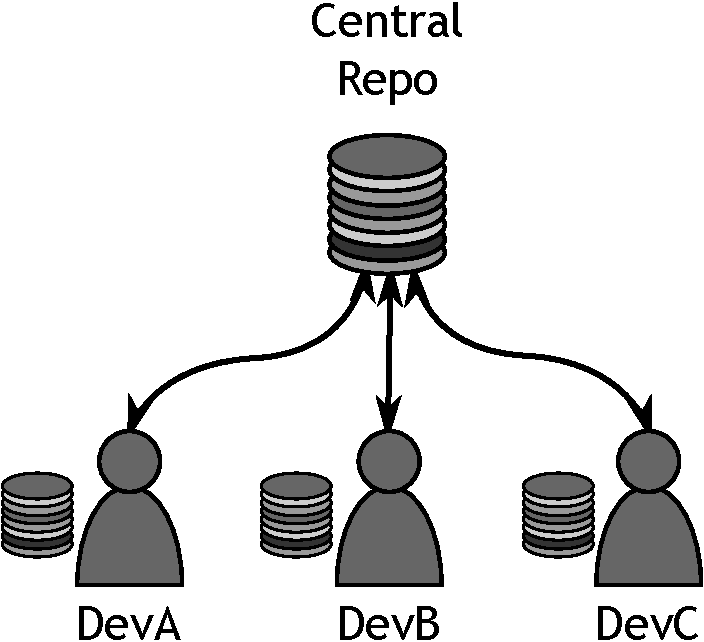
\includegraphics[width=7cm]{images/f-w1-d1.pdf}
	\caption{Centralised Workflow}
\end{figure}

\subsubsection{Integration Manager Workflow}
Der Integration Manager Workflow ist dem zentralisierten sehr "ahnlich, weil es auch hier ein \textbf{Blessed Repository} gibt, das jeder Entwickler als Referenz 
benutzt. Der Unterschied liegt darin, dass es nur eine Person gibt, welche die "Anderungen in das \textbf{Blessed Repository} einpflegt. Diese Person wird 
Integration Manager genannt.

Dieser Workflow funktioniert mit Git sehr gut. Entwickler arbeiten an ihrem lokalen Repository und sobald sie mit ihren "Anderungen zufrieden sind, laden sie ihre
Changes an einen Ort, wo sie der Integration Manger sehen kann. Dann begutachtet der Integration Manager die Ver"anderungen, die die Entwickler gemacht haben, und
kopiert sie in ein eigenes lokales Repository. Wenn dann alles wie geplant funktioniert, l"adt der Integration Manager die Changes in das Blessed Repository, so dass
alle anderen Entwickler zugriff auf den neuen Code haben. 

\begin{figure}[bt]
	\centering
	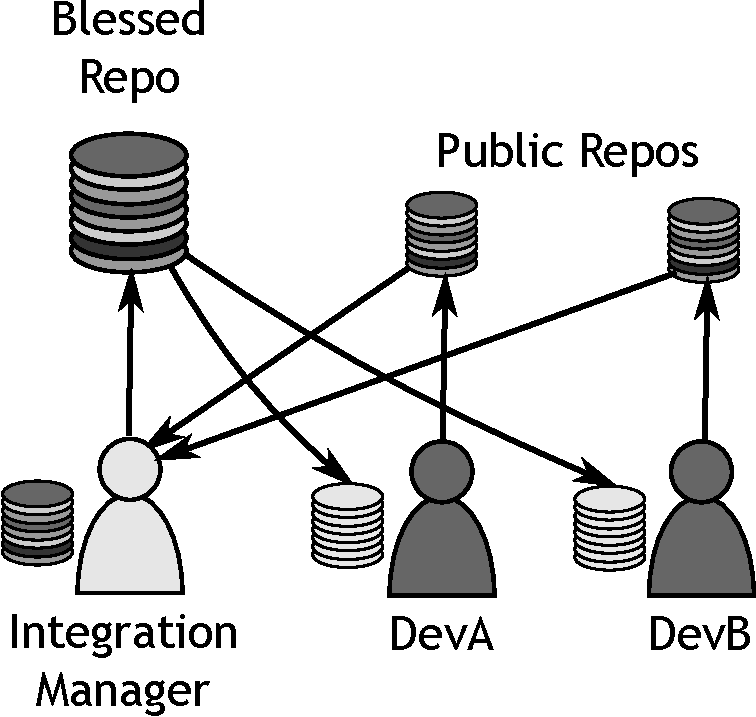
\includegraphics[width=7cm]{images/f-w1-d2.pdf}
	\caption{Integration Manager Workflow}
\end{figure}

\subsubsection{Dictator and Lieutenant Workflow}

Der Diktator und Leutnant Workflow ist sozusagen eine Erweiterung des Integration Manager Workflows. Er passt eher zu gr"o"seren Teams, wo Elemente oder Teile des
Codes einem \textbf{Leutnant} zugewiesen werden k"onnen, der daf"ur verantwortlich ist, jede "Anderung seines Bereichs abzusegnen.

Sobald die Leutnanten mit ihrem Code zufrieden sind, machen sie den Code dem Diktator zug"anglich. Dieser nimmt dann eine "ahnliche Rolle wie der Integration
Manager des vorigen Workflows ein. Schlussendlich werden alle Changes in das Blessed Repositpory gepusht, von dem die Entwickler mit weniger Rechten den Code beziehen
k"onnen.

\begin{figure}[bt]
	\centering
	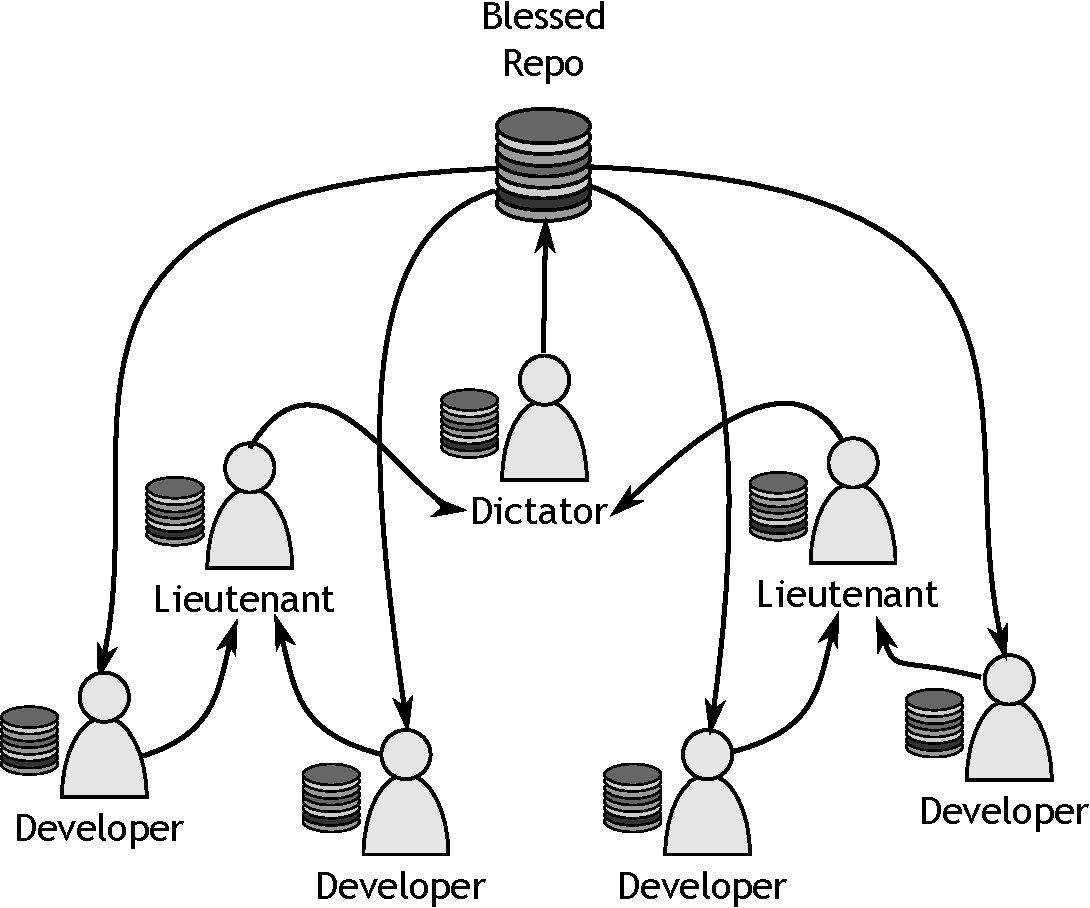
\includegraphics[width=7cm]{images/f-w1-d3.pdf}
	\caption{Dictator and Lieutenant Workflow}
\end{figure}

\begin{callout}{Terminology}{Blessed}
Ein Blessed Repository (oder Canonical) ist Repository, welches die Anerkennung des Projektmanagers hat. Es ist sozusagen der Standard, von dem alle anderen Kopien
gemacht werden. Wenn es einen Ort gibt, an dem der Code fehlerfrei sein sollte, dann im Blessed Repository. Falls Du Dein Projekt "offentlich zug"anglich machst,
wird das Blessed Repository f"ur gew"ohnlich das sein, auf das alle zugreifen k"onnen um es als Ausgangspunkt f"ur ihre Entwicklungen zu nehmen.
\end{callout}

Die Hauptsache, an die man sich erinnern sollte, ist, dass Git f"ur jeden dieser Workflows geeignet ist. Dadurch ist es ein sehr flexibles System, das es Dir
erlaubt, auf jedem dieser Wege zu arbeiten, wie auch immer Du Dich entscheidest. 

\subsection{Offline Committing}

Eines der n"utzlichsten und am meisten untersch"atzten Features eines dezentralen VCS ist wahrscheinlich das Offline Committing. Es ist vielleicht deswegen
untersch"atzt, weil nicht alle Versionsverwaltungssysteme "uber dieses Feature verf"ugen. Offline Committing bedeutet, dass man Dateien zum Repository hinzuf"ugen
kann, ohne mit einem zentralen Repository verbunden zu sein.

Wenn man reist, oder schlichtweg nicht im B"uro ist, k"onnen Entwickler und Integratoren dennoch damit fortfahren Code zu reviewen, die letzten "Anderungen
begutachten, Diffs anschauen und Code-"Anderungen in das Repository committen. All dies ist der Tatsache geschuldet, dass Git 99\% seiner Operationen lokal
ausf"uhrt. Wenn ein Repository kopiert wird, setzt Git lokal tats"achlich eine Kopie des kompletten Repositories auf, was den Entwicklern die Flexibilit"at gibt von
"uberall aus zu arbeiten, ohne dass Zugang zum Firmennetzwerk vorrausgesetzt wird. 

Sobald die Entwickler dann in ihr B"uro zur"uckgekehrt sind laden sie ihre "Anderungen einfach in das ``"offentliche'' Verzeichnis (sei es nun lokal oder ein
Blessed Repository) und alle Commits, die sie in ihrer Abwesenheit fertiggestellt haben, werden dem Rest des Teams inklusive der gesamten Historie und 
Zwischenst"anden zug"anglich gemacht

\subsection{Developer Interaction}

Eine Faktor, den man bei der Auswahl des zu verwendenden Versionsverwaltungssystems beachten sollte, ist der der Entwickler-Interaktion. Damit ist die Art und Weise gemeint, auf die die Entwickler das VCS benutzen und es bedienen. Es gibt vier Arten der Interaktion

\subsubsection{Graphical User Interface Client (GUI)}


Eine GUI erlaubt es dem Entwickler, oder Benutzer, das Repository in einer grafischen Oberfl"ache mit Maussteuerung zu ver"andern. Ein GUI-Client besteht normalerweise aus einer seperaten Anwendung, die gestartet wird, wenn ein User am Repository "Anderungen vornehmen will, zum Beispiel Dateien hinzuf"ugen oder Modifikationen committen will. 

Manche Entwickler ziehen einen extra Client f"ur die Interaktion vor, wohingegen andere es lieber m"ogen, wenn die Tools ineinander integriert sind.

\subsubsection{Shell Extension Integration}

Die Integration in die Shell macht es Entwicklern m"oglich, mit dem Repository so zu interagieren, wie sie es normalerweise beim modifizieren von Dateien und Ordnern auch tun w"urden. Eine der am meisten benutzten Shell-Erweiterungen f"ur Git ist TortoiseGit, welches sich selbst in den Windows Explorer integriert. Dadurch wird dem User erm"oglicht, durch einen Rechtsklick auf ein File in einem Git-Repository kontextsensitive Aktionen durchzuf"uhren.

\subsubsection{Command Line Interface (CLI)}

Das Kommandozeilen-Interface wird von vielen Entwicklern bevorzugt, da sie es skripten k"onnen und genau sehen, was geschieht - oftmals sehr viel dataillierter, als in einer GUI. Das Command Line Interface gibt einem vollst"andige Kontrolle "uber das Produkt, es ist ausserdem erw"ahnenswert, dass beinahe alle Versionskontrollsysteme ihr Leben als kommandozeilengesteuerte Programme begannen. Aber warum ist das so? Es braucht viel Zeit und Arbeit, alle Optionen und Kleinigkeiten in eine GUI zu integrieren! Das CLI wird fast immer das m"achtigste aller Tools sein, besonders dort, wo VCS betroffen sind. 

\section{Day 4 - ``Eine Entscheidung wurde gef"allt''}

\subsection{Die Vorraussetzungen pr"ufen}

Der wichtigste Aspekt bei der Wahl eines Versionskontrollsystems ist die Definierung der Vorraussetzungen. Diese k"onnen wenige sein, oder sie sind sehr speziell; aber lasst uns sehen, was John und sein Team f"ur die wichtigsten Anforderungen an ein VCS halten und wof"ur sie sich schlussendlich entschieden haben.

\begin{trenches}
``Es scheint, als w"are offline-committing eine sehr n"utzliche Sache. '' sagte Mike nickend. ``Besonders f"ur Leute wie John, die st"andig reisen.''

``Dem stimme ich zu, es w"are toll in einem Flugzeug sitzen zu k"onnen und trotzdem den gesamten Code zusammenf"ugen zu k"onnen, die History jedes Abschnitts zu kennen, '' antwortete John. ``Git scheint in Bezug auf das Branching auch sehr m"achtig zu sein.''

``In der Tat,'' schaltete sich Klaus ein, ``Ich nutze Branching zuvor in Subversion und es war ein Lebensretter. Git wird nachgesagt, dass es das auch sehr schnell bewerkstelligt.''

``Dank der Tatsache, dass Git scheinbar mehrere Arbeitsweisen unterst"utzt k"onnen wir sie ausprobieren, um zu pr"ufen, wie sie f"ur uns funktionieren.'' Markus schaute sein Team an. ``Also legen wir uns auf Git fest?''

Das Team nickte und jeder ausser John verliess den Meeting-Raum. Das versprach interessant zu werden, sehr interessant.
\end{trenches}

Da dieses Buch von Git handelt, werden wir nicht allzu tief auf die Funktionsweisen oder Features anderer VCS eingehen. Dieses Kapitel hat Dir hoffentlich genug Informationen gegeben um andere Versionskontrollsysteme auszuprobieren, falls  n"otig. Die Hauptsache, die man im Hinterkopf behalten sollte ist, dass Git ein dezentrales VCS ist. Deshalb ist es wichtig, daran zu denken, dass es mit den gleichen Workflows benutzt werden kann wie zentrale Systeme es tun.

Die Anforderungen von John und seinem Team sind nicht sehr speziell. Sie sind ein eher kleines Team, das die Vorteile eines gut organisierten Codes haben m"ochte. Au"serdem m"ochten sie ihre Team-Funktionen und die Dynamik einbringen, um sie an das Versionskontrollsystem anzupassen und es somit zum Kern ihrer Entwicklungsarbeit zu machen.

Versionskontrolle ist kein Ersatz f"ur einen guten Workflow. Es ist nicht erfunden worden, um alles besser zu machen. Wenn Du Leute in deinem Team hast, die nur ihr eigenes Ding durchziehen und sich nicht um ihre Arbeitsweise sorgen, wird ein VCS nicht auf einmal alles verbessern. Ein Tool ist nur ein Tool, und Versionskontrolle ist nichts anderes: Ein Tool. Du kannst dem unordentlichsten Baumeister eine sch"one neue Werkzeugkiste kaufen, aber solange er nicht den Willen hat sich zu "andern wirst Du feststellen, dass alle seine Werkzeuge im gr"o"sten Fach am Boden landen. 

\section{Day 5 - ``Arbeiten wie ein Team''}

\subsection{Team-Organisation}

Nun, da wir die Grundlagen behandelt haben, sehen wir uns an, wie John sein Team zusammengestellt hat, um herauszufinden, ob sie Versionskontrolle "uberhaupt einsetzen k"onnen. Es ist sehr wichtig, dass das team versteht wie das Modell funktioniert, was von ihnen erwartet wird und inwiefern sie Zugang zum Repository haben. Meistens werden die Leute frustriert, wenn sie nicht wissen, was sie tun oder eben nicht tun, oder weil sie keinen Zugriff auf bestimmte Teile des Codes haben.

\begin{trenches}
Es war 16:36 Uhr am Freitag und der Tisch im Meeting-Raum war voll mit leeren Cola-Dosen, Pizza-Schachteln und einer japanischen Obentobox, die einem besonders starrk"opfigen Mitglied des Teams geh"orte, der geschworen hatte, nie wieder Pizza zu essen. Es war Markus Idee gewesen, das Essen als Verst"arkung zu bestellen, um die Diskussion wieder gest"arkt fortf"uhren zu k"onnen. Das Team versuchte zu entscheiden, wie seine Organisation aussehen sollte.

``Es gibt also keine M"oglichkeit, eine Kombination von Modellen einzuf"uhren?'' fragte Mike.

``Ich sch"atze nicht,'' sagte John. ``An was hast Du denn gedacht?'' Seine Brille rutschte seine Stirn herunter und er wurde nun richtig m"ude.

``Nun, ich nehme an, dass wir die Software in zwei Teile aufgeteilt haben. Wir haben die Library, an der Klaus, Jack und ich arbeiten. Dann haben wir noch die grafischen Elemente, um die sich Simon, Martha und Rob k"ummern. Und ich kenne die Tools, die Eugene schreibt.'' Jeder h"orte nun Mike zu, als dieser fortfuhr: ``John, Du willst Dich nicht um die Libraries k"ummern m"ussen, weil das eher Klaus Part ist. Warum setzen wir also nicht zwei Integratoren ein? Klaus und Du selbst habt die Rechte um in das Blessed-Repository pushen zu k"onnen. John kann von von seinen Jungs pullen, wohingegen Klaus den Code von seinen Team-Mitgliedern bezieht. Schlussendlich haben wir ein gutes modell der Versionskontrolle.'' 

John hob seine Augenbrauen an, ``Nicht schlecht Mike,'' sagte er, sichtlich beeindruckt. Nachdem sie einige Stunden damit verbracht hatten, die verschiedenen Workflows durchzugehen und Zust"andigkeiten abzukl"aren, f"uhlte es sich nun gut an, endlich eine Entscheidung getroffen zu haben.

``Also fangen wir am Montag an?'' fragte Markus, der vom anderen Ende des Tisches zugeh"ort hatte.

``Allerdings!'' Verk"undete Klaus, ``Am Montag werden wir alle Gits!''
\end{trenches}
